%%% Architecture section

\section{Monitoring Architecture}
%There are many proposed architectures for use in runtime monitoring. Fundamental questions such as where the monitor executes (\eg, external hardware or on-system), what the monitor watches (\eg, memory values, executed instructions, etc.) and how the monitor obtains input (\eg, system instrumentation, external sensors) are dependent on both the properties of the system being monitored and the desired effects of monitoring (\ie, observation or enforcement/control).  

%% what are existing system architectures
Many modern safety-critical embedded systems are designed as distributed systems to provide the ability to meet the necessary reliability, fault-tolerance, and redundancy. The individual system components are typically connected via a network bus, of which there are many different common types \cite{Rushby2001}. %Controller Area Network (CAN) is a common bus for ground vehicles, being standard on automobiles and widely used in other systems.
%

\textit{Controller Area Network.} % add CAN citation?
Controller Area Network is a widely used automotive network developed by Bosch in the 1980s \cite{Bosch1991}. 
In this work we focus primarily on monitoring CAN because it is a common automotive bus which typically conveys enough of the state we wish to observe without instrumentation.
%
CAN is an event-based broadcast network with data rates up to 1Mb/s (although usually used at 125-500kbps). Messages on CAN are broadcast with an identifier which is used to denote both the message and the intended recipients. The message identifiers are also used as the message priorities for access control.

Although CAN is an event-based bus it is often used with periodic scheduling schemes so the network usage can be statically analyzed. Because of this our monitoring scheme is based on a time-triggered network sampling model, which allows it to monitor time-triggered networks as well.
%% old CAN paragraph, stealing above from background instead
%CAN is an event-triggered multi-master broadcast bus originally designed for automotive applications. Message arbitration utilizes a message-id based priority scheme and physical layer bit dominance to control bus access. CAN nodes take turns transmitting their messages onto the bus using the individual message identifiers as network priorities. In this way, the highest priority message that is ready to be sent at any given time is the message that gets sent.

%%% Cutting for space and redundancy (this is mostly said in intro, except risks of instrumentation on system behavior
%Existing runtime monitoring techniques tend to clash with the constraints imposed by safety-critical embedded systems. 
%Many existing monitors rely on automatic generation of instrumentation code or automated generation of the monitor itself (\eg, \cite{Havelund2004, Pike2011}).
%This is complicated when using external suppliers or black-box components due to the lack of source code access. Instrumentation also poses the risk of negatively affecting the non-faulty system behavior, especially timing in real-time systems.

As mentioned previously, existing runtime monitoring techniques which rely on code instrumentation are not directly applicable to systems with black-box components.
Instead of instrumentation, we propose a passive external bus-monitor which only checks system properties that are observable by passively observing system state from an existing broadcast bus.
%These include not only direct constraints including cost sensitivity and real-time computation but also development constraints such as system certification and source code access for black-box components.
We focus on ground vehicles and CAN buses specifically in this work, but other similar systems and broadcast networks can also be monitored using this approach.
%Although we focus on ground vehicles and CAN in this work, other similar systems can also be monitored with this approach due to the flexible interface and system model.
For example, safety-critical buses in star configurations which don't have a single bus line that can observe all traffic can be monitored by placing the monitor in the network's hub or by connecting multiple buses lines directly to the monitor. 
%For example, systems without a broadcast bus may be monitored by exposing the desired system state to the monitor (either through instrumentation or intelligent monitor placement such as network gateways/routers).

\begin{figure}[!h]
\centering 
%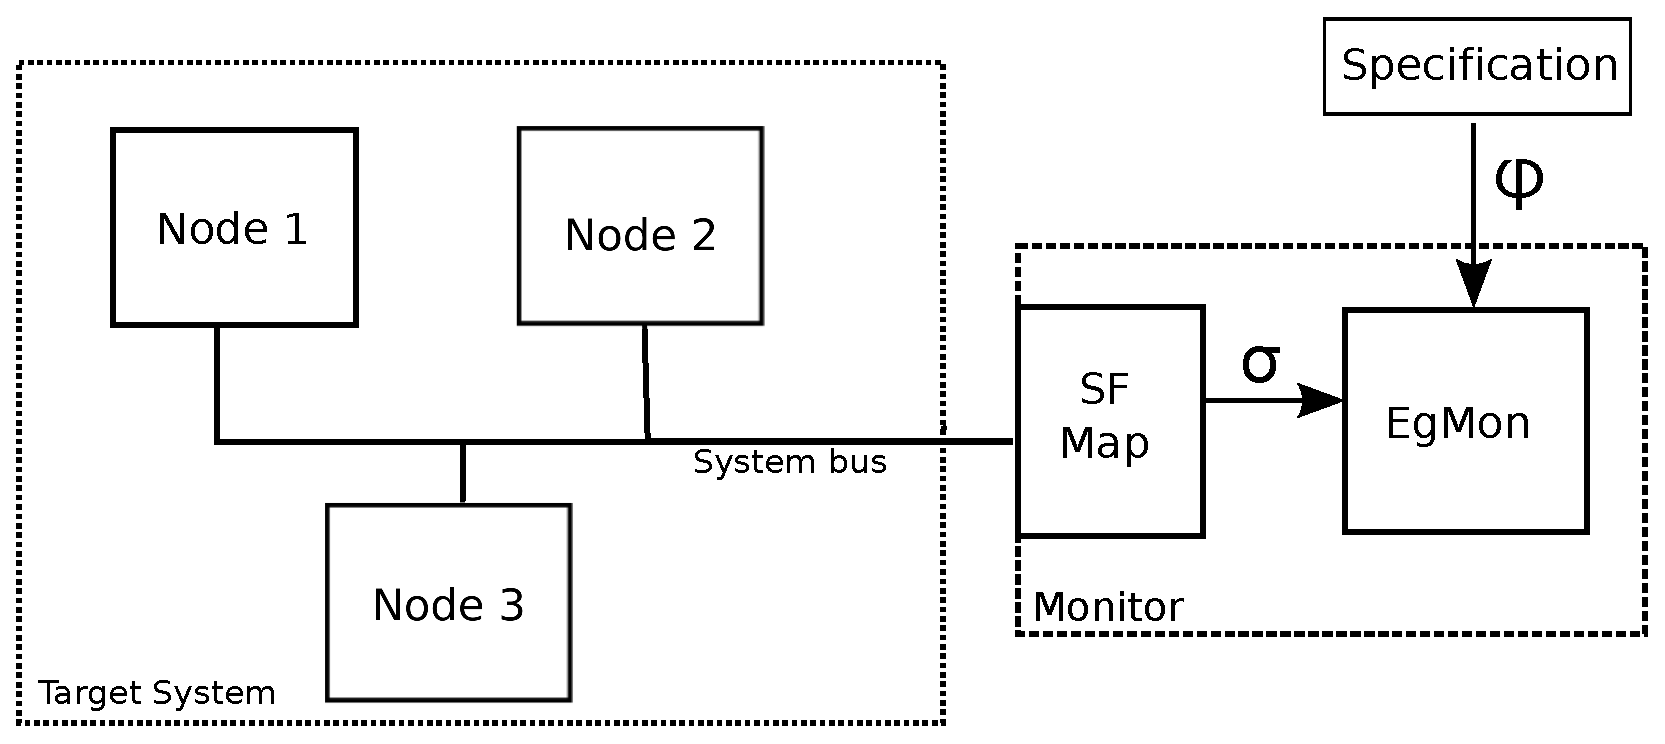
\includegraphics[width=4.5in]{img/newArch}
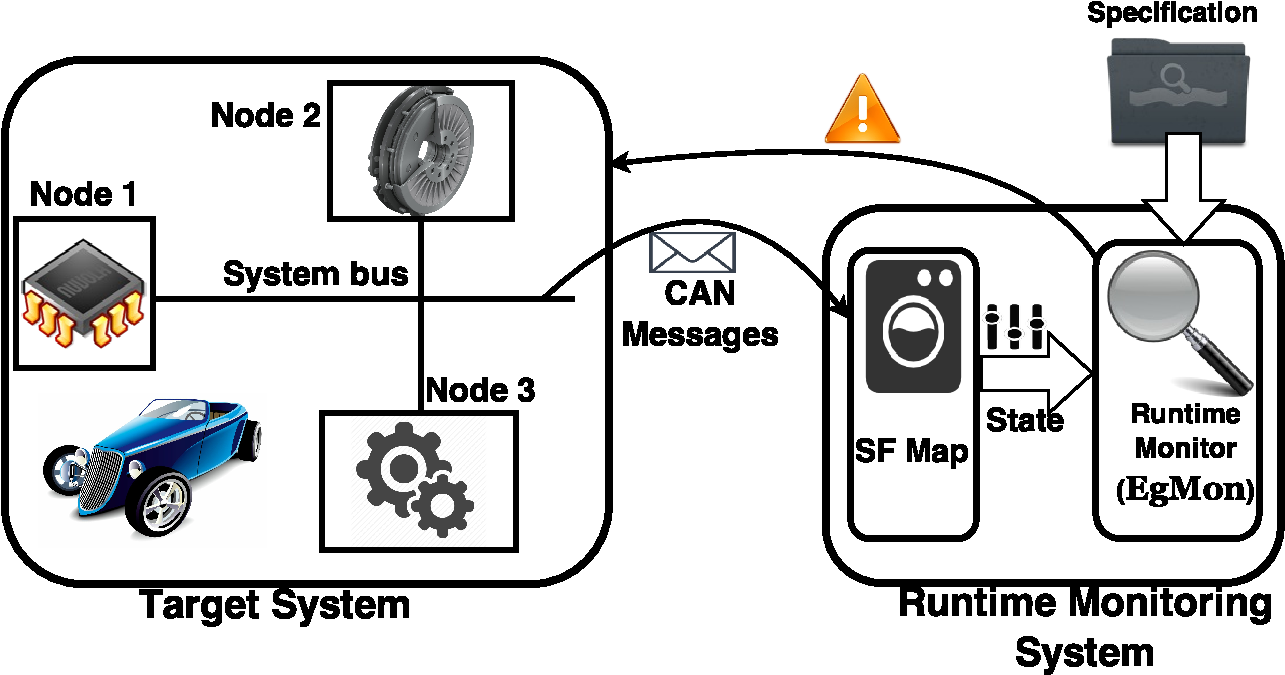
\includegraphics[scale=0.4]{img/ARV-main.pdf}
\caption{External monitor architecture outline \label{fig:architecture}}
\end{figure}


%\subsection{Architecture Outline}
An outline of our monitor architecture is shown in Figure \ref{fig:architecture}. 
The monitor is connected to the target system as an additional passive node on its broadcast bus. 
% sfmap paragraph
Different systems have varying specification needs which can not always be easily met within a formal specification language. 
In order to provide flexibility to map system state onto the formal specification language (in our case, in propositions) we provide a \sfmap interface which defines the mapping between the observed system state and the monitored specification. 
This type of interface is common in monitors for real systems, including MaC's filters \cite{Kim2004} and the AP evaluation filter from \cite{Heffernan2014}.
%% 
The monitor's \sfmap generates the system trace by building the necessary propositions based on the observed bus traffic. 
This generated trace is provided to the monitoring algorithm which checks it against the given system specification, outputting whether the trace violated or satisfied the specification at each trace step (subject to delays waiting on future  state).
%% took action controller out of arch picture so let's not mention it, could add it back in if we want...
%The algorithm's output is sent to an action controller which can perform the desired response to any specification violations, such as logging the violations or triggering a recovery action.

%\begin{figure}[!t]
%%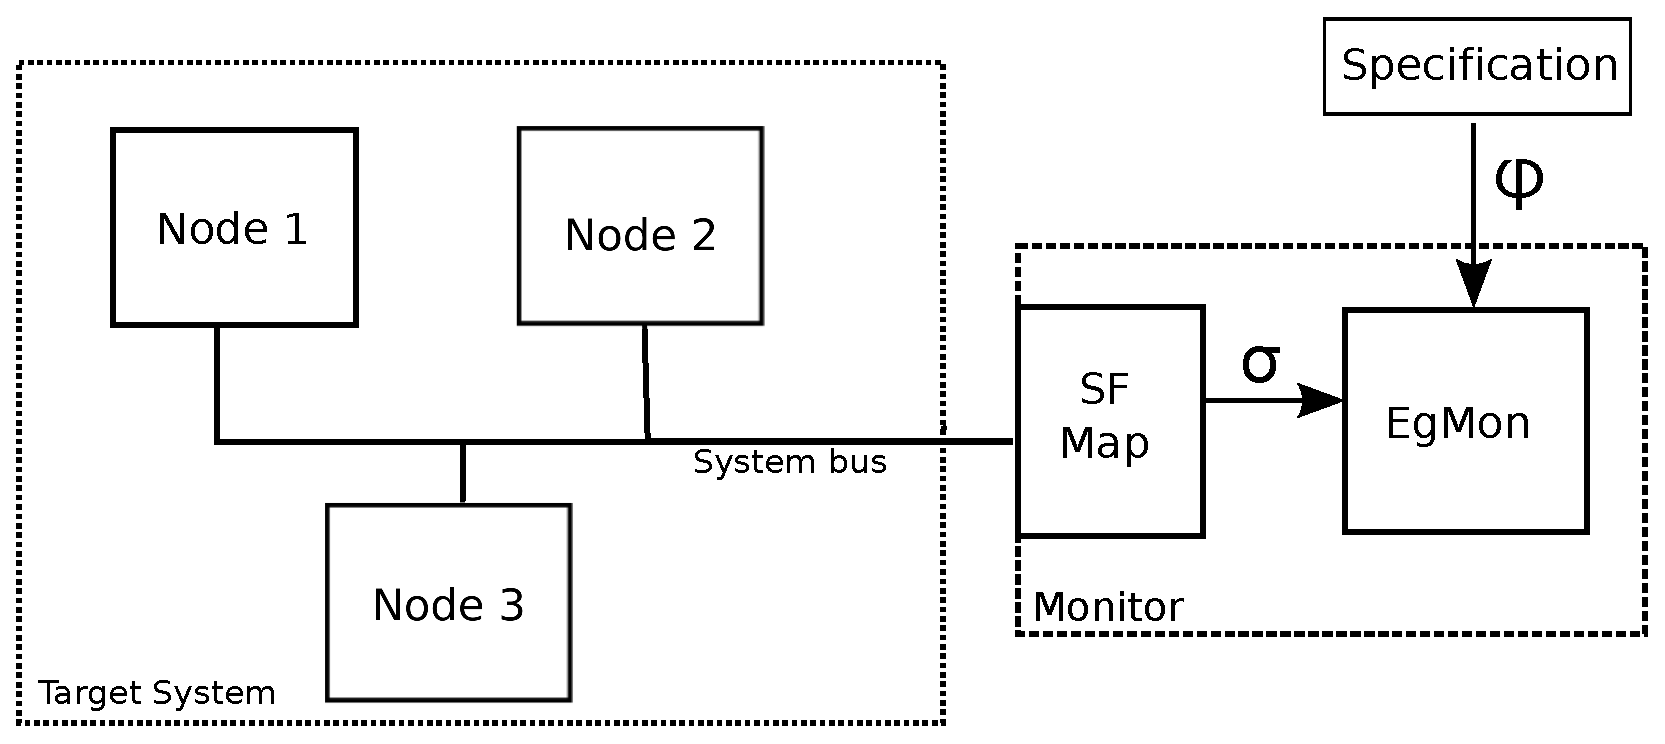
\includegraphics[width=4.5in]{img/newArch}
%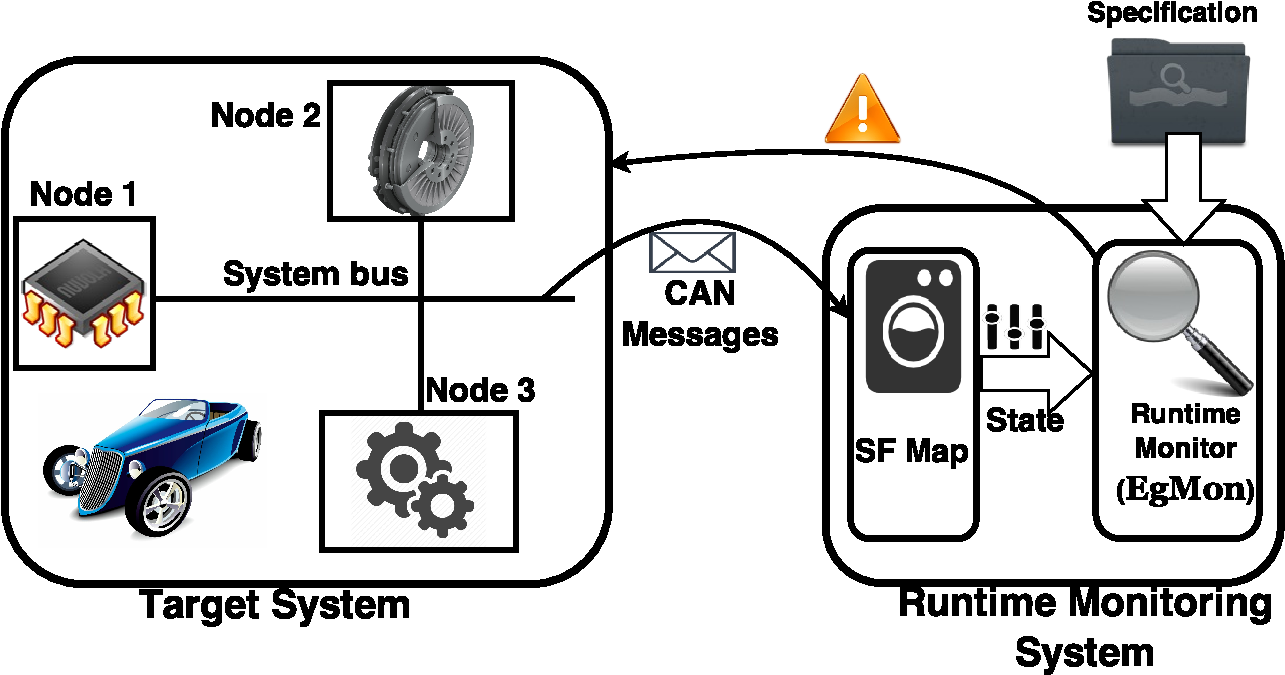
\includegraphics[scale=0.5]{img/ARV-main.pdf}
%\caption{External monitor architecture outline \label{fig:architecture}}
%\end{figure}

This architecture separates the lower-level system dependent configuration from the high-level system specification in a way similar to the architecture used in MaC \cite{Kim2004}.
%This architecture separates the system-independent formal aspects of the monitor from the system-dependent components including the system interface and action controller. 
%By utilizing a semi-formal interface, we can separate the formal aspects of the monitor, which are completely independent from the target system, from the more practical pieces: the monitor interfaces and their configurations, which are system dependent. 
This allows us to utilize a core formal monitoring algorithm and framework with any system where an \sfmap can be used to create a system trace.
Separating the system dependent and system-independent aspects of the monitor allows the high level system requirements be somewhat abstracted away from the implementation. 
This helps keep the monitoring specification matched closer to the system requirements documentation which usually does not include low-level implementation details. 
This architecture also makes the monitor more robust to changes in the target system.
If the system changes in a way that affects the monitoring-relevant messages, only the \sfmap configuration needs to be updated, rather than the monitor itself.
%This is a similar situation to the two-level specifications used in the MaC framework \cite{Kim2004}.

